% This file was created by tikzplotlib v0.9.8.
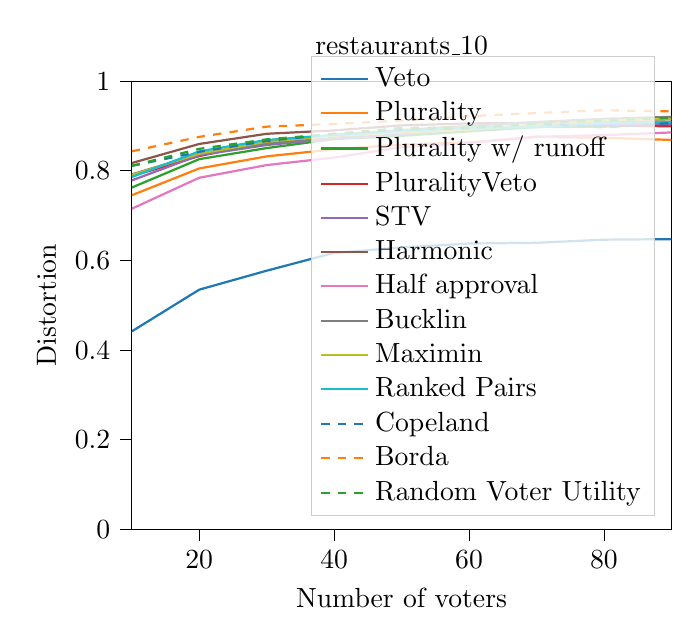
\begin{tikzpicture}

\definecolor{color0}{rgb}{0.12156862745098,0.466666666666667,0.705882352941177}
\definecolor{color1}{rgb}{1,0.498039215686275,0.0549019607843137}
\definecolor{color2}{rgb}{0.172549019607843,0.627450980392157,0.172549019607843}
\definecolor{color3}{rgb}{0.83921568627451,0.152941176470588,0.156862745098039}
\definecolor{color4}{rgb}{0.580392156862745,0.403921568627451,0.741176470588235}
\definecolor{color5}{rgb}{0.549019607843137,0.337254901960784,0.294117647058824}
\definecolor{color6}{rgb}{0.890196078431372,0.466666666666667,0.76078431372549}
\definecolor{color7}{rgb}{0.737254901960784,0.741176470588235,0.133333333333333}
\definecolor{color8}{rgb}{0.0901960784313725,0.745098039215686,0.811764705882353}

\begin{axis}[
legend cell align={left},
legend style={
  fill opacity=0.8,
  draw opacity=1,
  text opacity=1,
  at={(0.97,0.03)},
  anchor=south east,
  draw=white!80!black
},
tick align=outside,
tick pos=left,
title={restaurants\_10},
x grid style={white!69.0196078431373!black},
xlabel={Number of voters},
xmin=10, xmax=90,
xtick style={color=black},
y grid style={white!69.0196078431373!black},
ylabel={Distortion},
ymin=0, ymax=1,
ytick style={color=black}
]
\addplot [thick, color0]
table {%
10 0.4417
20 0.5348
30 0.5771
40 0.6169
50 0.6289
60 0.6377
70 0.6393
80 0.6463
90 0.6475
};
\addlegendentry{Veto}
\addplot [thick, color1]
table {%
10 0.7454
20 0.8052
30 0.8321
40 0.848
50 0.8584
60 0.8631
70 0.8757
80 0.8736
90 0.8688
};
\addlegendentry{Plurality}
\addplot [thick, color2]
table {%
10 0.7625
20 0.8259
30 0.8506
40 0.8706
50 0.8779
60 0.8879
70 0.8974
80 0.8982
90 0.9034
};
\addlegendentry{Plurality w/ runoff}
\addplot [thick, color3]
table {%
10 0.7882
20 0.8328
30 0.8637
40 0.8801
50 0.8901
60 0.8937
70 0.9012
80 0.9017
90 0.899
};
\addlegendentry{PluralityVeto}
\addplot [thick, color4]
table {%
10 0.7784
20 0.8347
30 0.8574
40 0.8719
50 0.8815
60 0.8941
70 0.9011
80 0.9051
90 0.9042
};
\addlegendentry{STV}
\addplot [thick, color5]
table {%
10 0.8172
20 0.8598
30 0.8825
40 0.8901
50 0.9012
60 0.9056
70 0.9068
80 0.9103
90 0.9096
};
\addlegendentry{Harmonic}
\addplot [thick, color6]
table {%
10 0.7153
20 0.7844
30 0.8127
40 0.8294
50 0.8527
60 0.8617
70 0.8759
80 0.8796
90 0.8855
};
\addlegendentry{Half approval}
\addplot [thick, white!49.8039215686275!black]
table {%
10 0.7919
20 0.8376
30 0.8602
40 0.8734
50 0.891
60 0.8999
70 0.9089
80 0.9158
90 0.9203
};
\addlegendentry{Bucklin}
\addplot [thick, color7]
table {%
10 0.7903
20 0.838
30 0.8648
40 0.8783
50 0.8855
60 0.892
70 0.9027
80 0.9121
90 0.9154
};
\addlegendentry{Maximin}
\addplot [thick, color8]
table {%
10 0.786
20 0.8432
30 0.8687
40 0.8799
50 0.8886
60 0.8965
70 0.8969
80 0.906
90 0.909
};
\addlegendentry{Ranked Pairs}
\addplot [thick, color0, dashed]
table {%
10 0.8109
20 0.8423
30 0.8663
40 0.8825
50 0.8918
60 0.8951
70 0.9049
80 0.8967
90 0.9066
};
\addlegendentry{Copeland}
\addplot [thick, color1, dashed]
table {%
10 0.8434
20 0.8756
30 0.8984
40 0.9044
50 0.9121
60 0.9216
70 0.9288
80 0.935
90 0.9326
};
\addlegendentry{Borda}
\addplot [thick, color2, dashed]
table {%
10 0.811
20 0.8489
30 0.8701
40 0.8823
50 0.8954
60 0.8972
70 0.9056
80 0.9124
90 0.9181
};
\addlegendentry{Random Voter Utility}
\end{axis}

\end{tikzpicture}
